\documentclass{clv3}

% Packages for template
\usepackage{hyperref}
\usepackage{booktabs}
\usepackage{multirow}
\usepackage{tikz}
\usepackage{pgfplots}
\usepackage{standalone}
\usepackage{xcolor}
\usepackage{standalone}
\definecolor{darkblue}{rgb}{0, 0, 0.5}
\hypersetup{colorlinks=true,citecolor=darkblue, linkcolor=darkblue, urlcolor=darkblue}


\usepackage{natbib}
\setcitestyle{aysep={,}} 
\bibliographystyle{newapa}
% Your packages here
\usepackage{graphicx}                % allow us to embed graphics files
\graphicspath{{figures/}{pictures/}{images/}{./}}
\usepackage{xcolor}
\usepackage{lipsum}
\usepackage{setspace}

\usepackage{pgfplots}
\pgfplotsset{compat=1.17}

\usepackage{listings}

%New colors defined below
\definecolor{codegreen}{rgb}{0,0.6,0}
\definecolor{codegray}{rgb}{0.5,0.5,0.5}
\definecolor{codepurple}{rgb}{0.58,0,0.82}
\definecolor{backcolour}{rgb}{0.95,0.95,0.92}

%Code listing style named "mystyle"
\lstdefinestyle{mystyle}{
  backgroundcolor=\color{backcolour},   commentstyle=\color{codegreen},
  keywordstyle=\color{magenta},
  numberstyle=\tiny\color{codegray},
  stringstyle=\color{codepurple},
  basicstyle=\ttfamily\footnotesize,
  breakatwhitespace=false,         
  breaklines=true,                 
  captionpos=b,                    
  keepspaces=true,                 
  numbers=left,                    
  numbersep=5pt,                  
  showspaces=false,                
  showstringspaces=false,
  showtabs=false,                  
  tabsize=1
}

%"mystyle" code listing set
\lstset{style=mystyle}



\def\thesistitle{DGS Glosses to German Text Translation Aided by Temporal Data}
\def\shorttitle{Thesis}
\def\yourname{Gijs Thissen}
\def\shortname{G. Thissen}
\def\yourprogramme{Cognitive Science \& Artificial Intelligence}
\def\yourcourse{Cognitive Science \& Artificial Intelligence}
\def\yourstudentnumber{2024993}
\def\finalmonth{May}
\def\finalyear{2021}
\def\supervisor{Dr. Dimitar Shterionov}
\def\committee{Dr. Sharon Ong}

\runningtitle{\shorttitle{}}
\title{\thesistitle{}}
\runningauthor{\shortname{}}
\studyinfo{\yourprogramme{}}{\finalyear{}}
\pgfplotsset{compat=1.15}
\begin{document}
\pagenumbering{gobble}
\thispagestyle{empty}

\begin{center}
\huge{\textbf{\thesistitle{}}} \\[1.2cm]
\normalsize{\yourname{}} \\
\normalsize{\textsc{Student number}: \yourstudentnumber{}} \\ [1cm]
\normalsize{\textsc{Thesis submitted in partial fulfillment}} \\
\normalsize{\textsc{of the requirements for the degree of}} \\
\normalsize{\textsc{Bachelor of Science in \yourprogramme{}}}\\
\normalsize{\textsc{Department of Cognitive Science \& Artificial Intelligence}} \\
\normalsize{\textsc{School of Humanities and Digital Sciences}} \\
\normalsize{\textsc{Tilburg University}} \\ [1.5cm]
\normalsize{Thesis committee:} \\[0.2cm]
\normalsize{\supervisor{}} \\
\normalsize{\committee{}} \\
\vfill
\normalsize{Tilburg University} \\
\normalsize{School of Humanities and Digital Sciences} \\
\normalsize{Department of Cognitive \ Science \& Artificial Intelligence} \\
\normalsize{Tilburg, The Netherlands} \\
\normalsize{\finalmonth{} \finalyear{}} \\
\end{center}

\newpage \thispagestyle{empty} \strut
\newpage \thispagestyle{empty}
%  NOTE: Please make sure to completely fill out the \def parts in meta-data.tex!

\section*{Preface}

Foremost, I would like to express my gratitude towards all persons that helped me during the creation of this thesis. From helping me with finding the topic to helping me correct my mistakes while programming the algorithms used in this thesis. 
\\

I would like to especially thank my research supervisor \textbf{Dr. Dimitar Shterionov} (Professor at Tilburg University) for the guidance given by helping me both with the research for this topic and correcting my many mistakes while coding. 

I am grateful to my fellow Thesis colleagues \textbf{Stan van der Vossen} (CSAI-Student) and \textbf{Jakob E. Hauser} (CSAI-Student) for the advice, translating sporadic German to English, and guidance given towards solving the problems I faced during the creation of this Thesis paper.

Lastly, even though they are unaware of me writing this Thesis paper, I would like to express my gratitude towards all the researchers that aided in the creation of the DGS-Korpus and especially by making it available online to the public.

\newpage \thispagestyle{empty} \strut
\newpage \pagenumbering{arabic}

\title{\thesistitle{}}
\author{\yourname}

\maketitle % Yes, again

\begin{abstract}

\end{abstract}

\section{Introduction}

\subsection{Deaf communication}

\subsection{Study of sign language}
early linguistics vs early sign language study

\cite{stokoe2005sign}
sign language us actually a language

GLOSSES

\subsection{Machine Translation}
basic NMT and NLP

\subsection{LSTM and Transfomer architecture}
zowel basic lstm en transformer

\subsection{Research Question}

\textbf{To what extent does temporal data aid in the performance of a machine translation system for sign language glosses to text?}

\begin{itemize}
    \item \textbf{How to introduce temporal data to the Machine Translation system?} \\
    The baseline system does not have temporal data added to it. This sub-question is related to how to add temporal data to the machine translation system.
    \item \textbf{To what extent does temporal data aid a Machine Translation system when compared to a baseline system?} \\
    The chosen dataset \cite{dgscorpus_3} contains both the glosses (i.e.: TO-HAVE-BSL1, I1\textasciicircum, BUTTER1A) and the timestamps next to them to indicate when and how long these signs have taken place. This sub-question is related to combining this temporal data with the baseline system. Both the baseline and the temporal experiments are described in the methods section.
    \item \textbf{To what extent does adding extra tokens have an effect on the performance of the Machine Translation system} \\
    The dataset contains both glosses on sign language and data on what the subject said during the interview (vocal). This sub-question is related to:
    \begin{enumerate}
        \item Combining the additional vocal data with the baseline system.
        \item Combining the additional vocal data with the temporal data and the baseline system.
        \item Measure to what extent does adding extra tokens have an effect on the performance of the Machine Translation system.
    \end{enumerate}.
\end{itemize}

\section{Related Work}

\subsection{Transformers}
machine translation en transformers

\subsection{Sign Language Translation}

papers die hier precies mee te maken hebben





\section{Data}

\subsection{Source}

The data consists of $405$ EAF-files (ELAN Annotation Files) gathered by the Institute for German Sign Language and Communication of the Deaf at Hamburg University \cite{prillwitz2008dgs}. These files consist of a total of $50$ hours of annotated recordings spanning a wide range of narrations regarding the cultural aspects of the deaf community. The interviews were conducted using a peer-to-peer procedure, where participant change roles according to the conversation \cite{prillwitz2008dgs}. During a discussion $2$ German Sign Language or Deutsche Gebärdensprache (DGS) signers conversed. Each conversation consisted of a standardized interview covering linguistical and social data \cite{deaf_areas}. Following this conversation, a spontaneous conversation on a given topic was held while the participants were encouraged to use as much basic vocabulary as possible \cite{deaf_areas}. In the EAF-files the signers are annotated as either Speaker A or Speaker B. The data was collected between January $2010$ and December $2011$  by videotaping $330$ participants from all $16$ Federated States (Bundesländer). The recordings were conducted using a mobile field lab in:

\begin{itemize}
  \item Areas with a relatively high deaf population density (deaf schools, deaf centres, and deaf institutes). \cite{age_data_hamburg} \cite{deaf_areas}
  \item The catchment areas of the former Schools for the Deaf.\cite{age_data_hamburg} \cite{prillwitz2008dgs}
  \item Areas which were easy to reach from surrounding rural communities. \cite{age_data_hamburg} \cite{deaf_areas}
  \item Areas that were suspected of having a distinct dialect. \cite{age_data_hamburg} \cite{prillwitz2008dgs}
\end{itemize}

 The data was collected by representatives of the local deaf community to take into account the regional varieties of DGS \cite{deaf_areas}. As can be seen in \autoref{fig:bundeslander} the data was sampled from participants across different age groups \cite{age_data_hamburg}. 


% Age category figure
\pgfplotstableread[row sep=\\,col sep=&]{
    interval & carT & carD \\
    18--30     & 12.1  & 12.4  \\
    31--45     & 13.6 & 13.9  \\
    46--60   & 12.7 & 12.4 \\
    61+   & 11.5 & 11.2 \\
    }\mydata

\begin{figure}[h]
\begin{tikzpicture}
    \begin{axis}[
            ybar,
            title={Age distribution in The DGS-Korpus project sample (Percentage Vs. Age Categories)},
            bar width=.6cm,
            width=.8\textwidth,
            height=.5\textwidth,
            legend style={at={(0.5,1)},
                anchor=north,legend columns=-1},
            symbolic x coords={18--30,31--45,46--60,61+},
            xtick=data,
            nodes near coords,
            nodes near coords align={vertical},
            ymin=0,ymax=25,
            xlabel={\/Age categories},
            ylabel={\/Percentage of participants (\%)},
        ]
        \addplot table[x=interval,y=carT]{\mydata};
        \addplot table[x=interval,y=carD]{\mydata};
        \legend{Male, Female}
    \end{axis}
    
\end{tikzpicture}
\caption{Showing the percentage of participants per age , divided into both the Male (shown in Purple) and Female (shown in Red) gender,  that participated in the creation of the DGS corpus (both annotated and non-annotated). \cite{age_data_hamburg}}
\label{fig:bundeslander}
\end{figure}

\subsection{ELAN}
The conversation conducted between the representatives of the deaf community has been annotated and stored in EAF-files. These EAF-files can be shown and edited using the ELAN software \cite{crasborn2008enhanced}. ELAN is a multimedia annotation software developed by \citep{elan_software} to assist in Linguistical studies, language conservation, and sign language research \cite{brugman2004annotating}. The software can be used to add annotations to video and/or audio recordings. An annotation can be a sentence, word, or in the case of sign language, a gloss. Using ELAN multiple annotations can be created that are sorted into tiers \cite{crasborn2008enhanced}.  

% EAF-example
\begin{figure}[h]
 \centering 
 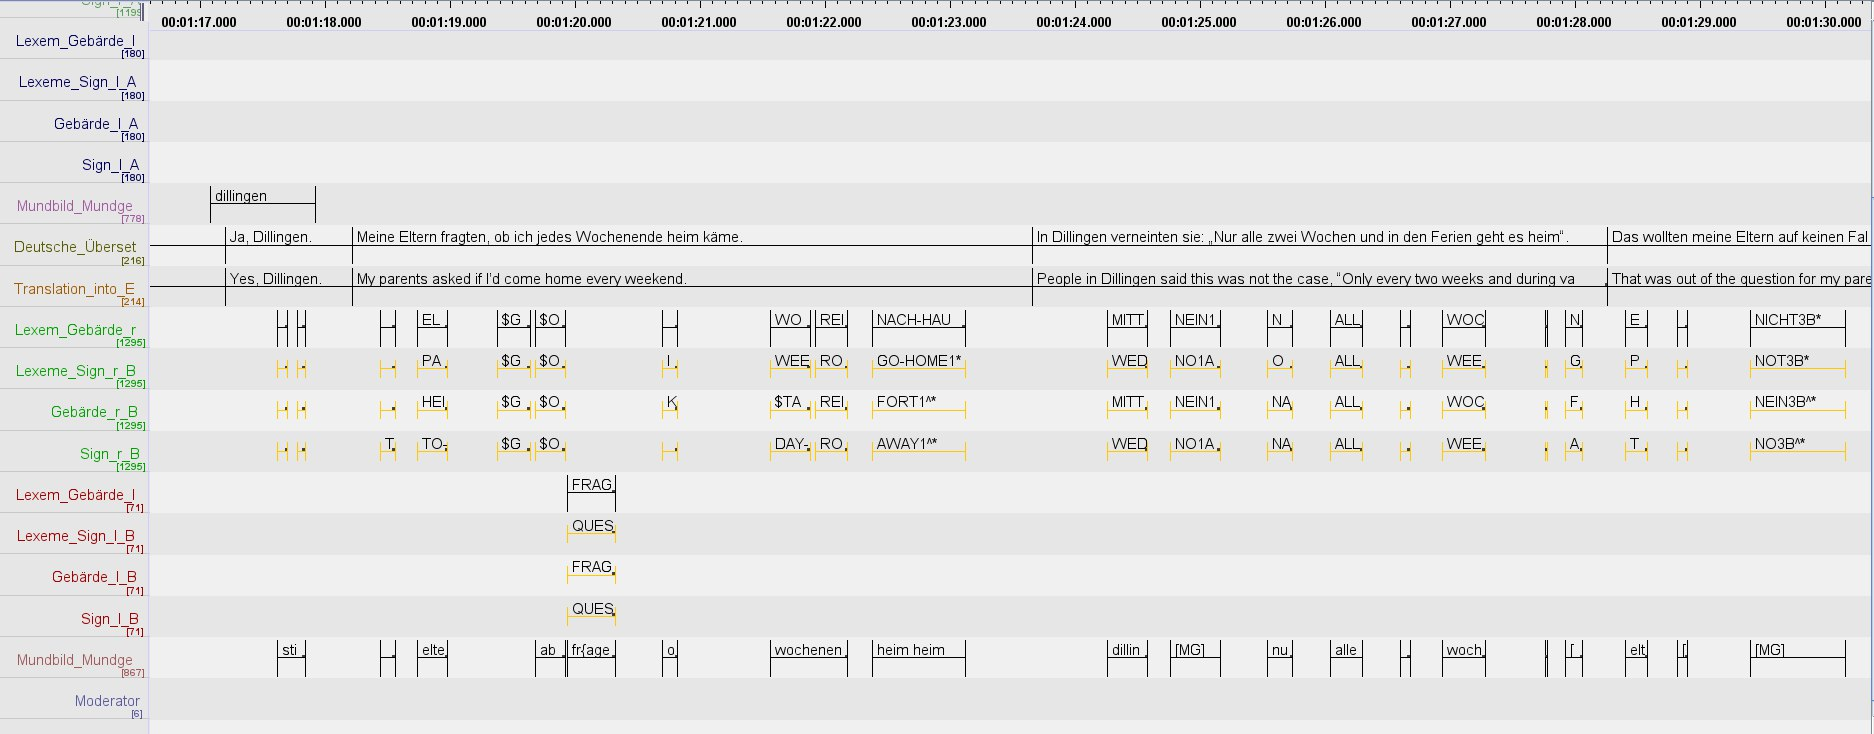
\includegraphics[width=14cm]{Bachelor CSAI thesis template/images/ELAN_example.jpg}
 \caption{Showing the structure of one of the EAF (English Annotated File)-files \cite{elan_example} inside the program ELAN. ELAN is a multimedia annotation tool used for multi-modality research \cite{sloetjes2017elan}. }
 \label{fig:elan_example}
\end{figure}

\subsection{Initial Translation}

The annotations divided into tiers are presented across a timeline. As can be seen in \autoref{fig:elan_example}these files are divided into $11$ different tiers, presented in both English and German due to accessibility \cite{konradoffentliches}. Take "Lexem\_Gebärde\_r\_A" for example, this tier is translated into English as "Lexeme\_Sign\_r\_A". The tiers present in the EAF-files, translated into English, are: "Time", "Sign\_l\_B", "Sign\_r\_B", "Lexeme\_Sign\_l\_B", "Lexeme\_Sign\_r\_B", 
"Translation\_into\_English\_B", "Sign\_l\_A", "Sign\_r\_A", "Lexeme\_Sign\_l\_A", "Lexeme\_Sign\_r\_A", and "Translation\_into\_English\_A" \cite{sloetjes2017elan}. The goal of this paper is to, through experimentation, show to what extent temporal data aids in the performance of a machine translation system for sign language glosses to text. For this purpose, both the German Sign Language and the German Language were chosen respectively. Since the target language is German it was decided to use the original glosses and translations that were available in the corpus.

The initial translation of the glosses in the data set (i.e.: Sign\_l\_A to Translation\_into\_English) was conducted by contracted sign language translators and interpreters \cite{konradoffentliches}. These researchers translated the data set word-for-word. Consequently, university students created coherent meaningful sentence like structures. Lastly, these sentences were fed back into the system until the proper meaning was determined by the DGS experts (\autoref{fig:uselesspipeline}) \cite{konradoffentliches}.

\begin{figure}[h]
 \centering 
 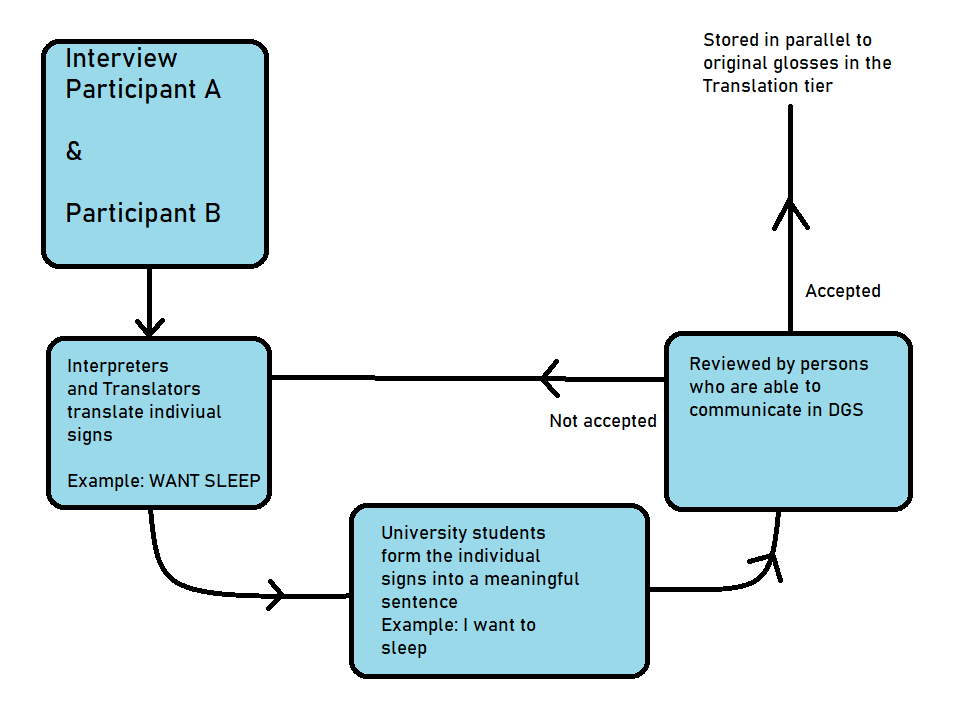
\includegraphics[width=14cm]{Bachelor CSAI thesis template/images/translation_pipeline.png}
 \caption{Showing the translation pipeline of the initial translation phase as conducted by the Institute for German Sign Language and Communication of the Deaf at Hamburg University. \cite{konradoffentliches} }
 \label{fig:uselesspipeline}
\end{figure}

\subsection{Segmentation}

As with spoken languages, sign languages tend not to have a naturally occurring white space character \cite{hankesegmentation} \cite{konradoffentliches}. Thus it is difficult to determine where a sign begins and where a sign ends. In this situation, the segmentator has two options: either add a gap or none at all. Unlike spoken languages, when a participant is signing two words, take TREE (rest your right forearm upon your left palm and twist) \cite{perniss2007space} and COW (make two horns using your thumb and little finger on top of your head), for example. There is a transitional period where the participant moves his or her arm from one sign to the next. When adding a gap between the signs, the segmentator determines that the transitional movements are not part of the token's form \cite{konradoffentliches}. Taking this into account researchers at the University of Hamburg have decided that for the creation of the DGS corpus gaps will be added. The direct result of this decision is located in the EAF files, where there is temporal data with no associated annotations.

\subsection{Lemmatisation and Gloss conventions}

When creating a corpus there is an intrinsic need to have conventions in place to make sure a uniform dataset is created. \cite{konradoffentliches} Therefore it is necessary to employ linguistics to standardise glosses using gloss conventions: \cite{kristoffersen2016designing}

\begin{itemize}
    \item In the field of Linguistics or more specifically in the field of lexicography, a lexical item forms the basic element of the lexicon of a language. Lexical signs are treated as items, that is as units of their respective sign language that would be found in the dictionary \cite{konradoffentliches}. When a deaf person signs SQUARE1\textasciicircum  it may mean different things such as a map, a recipe, or a page. In DGS \cite{perniss2007space} and several other European Sign Languages signs are iconically motivated \cite{pietrandrea2002iconicity} \cite{oomen2017iconicity}, meaning that there is a similarity between the form of the sign and the meaning of the sign. In the DGS corpus, type glosses are given an indication of iconic value by using a circumflex at the end: "SQUARE1\textasciicircum ". Examples of child types to the SQUARE1\textasciicircum parent type are: FORM1, MIRROR2, and PAPER4, these and all other non-circumflex glosses are subtypes. The numbers denote different lexical variants.
    \item Fully iconically motivated signs, also known as poly-morphemic signs, are denoted as productive signs in contrast to lexical signs that denote something instead of meaning. Productive signs, therefore, have a \$PROD token \cite{konradoffentliches}
    \item Due to the anonymisation laws present in Germany, where this corpus was created, all names are replaced by "\$NAME". Except when it concerns a famous person the \$NAME gloss is followed by the person's name. \cite{konradoffentliches}
    \item Foreign language elements are represented using the INTS token, for example, when signing the English word Germany instead of "Deutschland" it has been written as GERMANY-INST1.\cite{konradoffentliches}
    \item In German Sign Language it is conventional to use a one-handed manual alphabet, for example when spelling out someone's name. For these situations, the \$ALPHA token is used. Numbers are presented similarly by using \$NUM. \cite{konradoffentliches}  
\end{itemize}

Taking into account these points a uniform corpus was created with annotated signs presented on a timeline. An example of an annotated DGS sentence can be seen in \autoref{fig:sentence_example}.

\begin{figure}[h]
 \centering 
 
\includegraphics[width=14cm]{Bachelor CSAI thesis template/images/sentence_example.png}
 \caption{Showing an example sentence of the annotated corpus in DGS glosses. The German translation of this gloss sentence is: "Und dann fällt es einem wieder auf, dass der andere noch Fehler macht" \cite{dgscorpus_3}. (English translation: And then one notices again, that the other (person) is still making mistakes). 1. A token denoting a gesture. 2. The sign annotated as NM has iconic meaning. 3. One of several lexical variants of the lexical unit FEHLER.}
 \label{fig:sentence_example}
\end{figure}

\section{Methods}

\subsection{Experiments}

There are $4$ experiments to be carried out. \autoref{fig:baseline_comparison}

\subsubsection{Baseline}

To the baseline the other experiments will be compared. This model lacks any external added tokens. It consists of the glosses formed into a sentence as the source and their German translations as the target (Source: PRIVAT1A* FAMILIE1 Target: Privates oder Familie? \cite{dgscorpus_3}). The sign language glosses are without any transitional periods (See the Lemmatisation and Gloss conventions section in Data) and adhere to the standard gloss conventions.


\subsubsection{Temporal}

A sub-goal of this thesis-paper is to, through experimentation, show to what extent temporal data aids in the performance of machine translation systems for sign language glosses to text. This will be tested in the Temporal experiment. The data in the temporal experiment consists of the glosses formed into a sentence with tokens added to each word separated by a "|" character, e.g.: FAMILIE|120. The number behind the "|" character represents the total amount of milliseconds it took for a sign to be signed, in the given example this would mean that the sign for FAMILIE (English: Family) would have taken 120 ms to be made. As mentioned before these sentences are without the transitional periods from one sign to another (See the Lemmatisation and Gloss conventions section in Data). The "|" sign is a library standard sign to split Word features from the actual words \cite{klein-etal-2017-opennmt}. The temporal data files consist of glosses formed into a sentence with added temporal data and their German translation as the target (Source: PRIVAT1A*|340 FAMILIE1|460 Target: Privates oder Familie? \cite{dgscorpus_3})

\subsubsection{Vocal}

Another sub-goal of this thesis paper is to show to what extent adding extra tokens aids in the performance of machine translation systems for sign language glosses to text. This will be tested in both the Vocal and the Combined experiment. The data in the vocal experiment consists of glosses formed into a sentence with tokens added to each word that represent the spoken words uttered by the participant while performing this sign. Research has shown that the mouthing a deaf-person performs is of importance for the meaning of the sign that is being performed at the same time \cite{kristoffersen2016designing}. The spoken word and the gloss will be separated by the "|" character as per library standard \cite{klein-etal-2017-opennmt}. When using the OpenNMT library \cite{klein-etal-2017-opennmt} it is necessary that all source word features have the same amount of features. Thus when a sign does not have an accompanied mouthing a "nan" will be added instead of the spoken word. This is done to represent the empty space created by the empty row. The vocal data files consist of glosses formed into a sentence with added vocal data and their German translation as the target (Source: PRIVAT1A*|privat FAMILIE1|familie Target: Privates oder Familie?). It is important to note that all vocal word features are denoted solely using lowercase characters.

\subsubsection{Combined}

Research has shown that talking speed is affected by emotions \cite{kshirsagar2002multilayer}. The combination experiment is an experiment that combines the previously mentioned temporal and vocal features into one model.  The data will be seperated by a "|" and be processed in a GLOSS|vocal|TIME format. The same conditions apply on the combined model as applied on the vocal and temporal model. The combined data files consist of glosses formed into a sentence with added vocal and temporal data and their German translation as the target (Source: PRIVAT1A*|privat|340 FAMILIE1|familie|460 Target: Privates oder Familie? \cite{dgscorpus_3}).

\begin{figure}[h]
 \centering 
 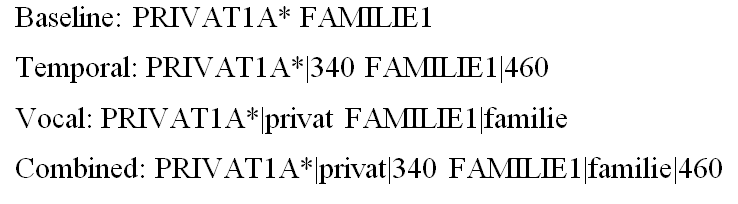
\includegraphics[width=14cm]{Bachelor CSAI thesis template/images/baseline_compared.PNG}
 \caption{Showing the source file textual comparison between the Baseline, Temporal, Vocal, and Combined experiments. In the temporal experiment the concept of time is added (in ms). In the vocal experiment the concept of spoken words is added (in lowercase letters). In the combined experiment these are combined into one.}
 \label{fig:baseline_comparison}
\end{figure}


\subsection{Pre-Processing}

\subsubsection{EAF to CSV}
Using the ELAN software $7$ of the $11$ tiers were selected and converted into a CSV file. This creates $2$ distinct CSV files that were consequently merged (\autoref{apx:first}). Due to having merged the files, there are no longer multiple persons in the data set, instead, the data set has transformed into a contextless database. Due to being able to access the timeline in ELAN \cite{elan_software}, it is possible to extract the temporal features of a given annotation. As mentioned before the annotators decided to add gaps between the signs \cite{hankesegmentation} \cite{konradoffentliches}, this has been carried over into the EAF-files, resulting in empty rows inside the CSV file. These need to be removed since the program automatically puts white spaces between words instead of pasting them into one giant string (\autoref{apx:first}). Failing to do so would result in temporal features being assigned to empty strings (A temporal-annotated sentence without removal of prior white spaces would result in \$GEST-NM\textasciicircum|430 |230 FEHLER1*|450 |400 \$GEST\textasciicircum|400).

\subsubsection{Data splitting}

After merging the data, the dataframe contains $5$ columns. As has been described $4$ experiments are to be performed: Sign, Temporal, Vocal, and Combined. For each of these experiments two files are need: a Source file (.src) , and a Target file (.trg). These files are fully extracted from the dataframe. By isolating the sentences in the dataframe it is possible to create a separate sentence set for every sentence. This will result in $5$ files: normal.en, vocal.en, times.en, combined.en and sentences.nl. "sentences.nl" is the target file for all the experiments and is therefore uniform.

To tokenize and split the data the \texttt{train\_test\_dev.py} (SOURCE NEEDED) script was used to both tokenize and split the data into a training, a validation, and a testing file. Since the data set only has $60000$ sentences it was decided to split the data into only 500 sentences for validation and testing each.  



\subsubsection{BPE}

\subsection{OpenNMT}
 preprocessing
limitations for token adding (elk woord heeft hetzelfde aantal tokens nodig)

\subsection{Parameters and Architecture}

\begin{table}[h]
\centering
\begin{tabular}{|ll|ll|}
\hline
\multicolumn{1}{|l|}{Parameter} & Setting     & \multicolumn{1}{l|}{Parameter} & Setting              \\ \hline
Encoder type                    & Transformer & Batch size                     & 1024                 \\
Decoder type                    & Transformer & Batch type                     & tokens               \\
Transformer feed-forward        & 2048        & Normalization                  & tokens               \\
Layers                          & 6           & Warm-up steps                  & 8000                 \\
Heads                           & 8           & Training steps                 & 20000                \\
RNN size                        & 512         & Validation steps               & 1000                 \\
Word embedding size             & 512         & Label smoothing                & 0.1                  \\
Position encoding               & True        & World size                     & 1                    \\
Maximum generator batches       & 2           & GPU rank                       & 0                    \\
Dropout probability             & 0.1         & Early stopping                 & 5                    \\
Optimization method             & adam        & Early Stopping criteria        & perplexity, accuracy \\
Adam beta2 parameter            & 0.998       & Max gradient norm              & 0                    \\
Decay Method                    & noam        & Parameters initialized at      & 0                    \\
Learning rate                   & 2           & Parameters\_init\_glorot       & True                 \\ \hline
\end{tabular}
\caption{Showing the parameters used for training using the Transformer architecture.The batch size is small since the GPU used for training had only 4GB of VRAM (NVIDIA GTX 980).}
\label{tab:parameter}
\end{table}

\subsection{BLEU}

BLEU is short for Bilingual Evaluation Understudy and is an evaluation metric for Neural Machine Translation. \cite{papineni2002bleu} 

\subsection{TER}


\section{Results}

\begin{table}
    
    \label{tab:results}
    \begin{tabular}{llrr}
        \toprule
                                                                  
        Word-Form                   &  Models                           &  BLEU                & TER    \\ 
        \midrule
        \multirow{3}{*}{Original}  &  Baseline                              &   \textbf{3.69}      &  \textbf{0.960} \\
                              & Temporal                                &   2.85               &  0.971 \\
                              & Vocal                                   &   2.03               &  1.000 \\
                              & Combined (Temporal + Vocal)             &   1.69               &  0.973 \\
    
        
    \end{tabular}
    \caption{SCHRIJF HIER NOG IETS}
\end{table}

\pgfplotstableread[row sep=\\,col sep=&]{
    Model & carT & carD \\
    Baseline     & 3.69  & 0.960  \\
    Temporal     & 2.85 & 0.971  \\
    Vocal   & 2.03 & 1 \\
    Combined   & 1.69 & 0.973 \\
    }\mydata

\begin{figure}[h]
\begin{tikzpicture}
    \begin{axis}[
            ybar,
            title={Experimentation Results (Score vs. Model)},
            bar width=.6cm,
            width=.8\textwidth,
            height=.5\textwidth,
            legend style={at={(0.5,1)},
                anchor=north,legend columns=-1},
            symbolic x coords={Baseline, Temporal, Vocal, Combined},
            xtick=data,
            nodes near coords,
            nodes near coords align={vertical},
            ymin=0,ymax=4,
            xlabel={\/Models},
            ylabel={\/Score},
        ]
        \addplot table[x=Model,y=carT]{\mydata};
        \addplot table[x=Model,y=carD]{\mydata};
        \legend{BLEU-score, TER-score}
    \end{axis}
    
\end{tikzpicture}
\caption{Showing the results from the $4$ performed experiments. On the X-axis the different models are presented. On the Y-axis the score is shown (for the meaning of the TER and BLEU score: see their respective sections.)}
\label{fig:results_graph}
\end{figure}

\section{Discussion}

gebarentaal dialect neit meegomen

schrijf een stuk over wat er gebeurt als je dat hele ding standardised

\section{Conclusion}


\newpage
\bibliography{mybib}

\newpage
\appendix

\appendixsection{Merging Code} \label{apx:first}
\begin{lstlisting}[language=Python, caption=Shown is the Python code to merge the multiple CSV-files into one DataFrame.]
class create_file(object):
    def __init__(self, path="datasets/"):
        self.path = path
        self.inputs = listdir(str(path))
        self.dataframe = self.drop_empty()

    def clean_dataframe(self, dataset):
        """
        Load the dataset into a frame, delete the "Unnamed" column,
        and replace all instances of nothing with a numpy nan.
        Requires the numpy library.

        :param dataset: str, input name of the dataset.csv
        :return: dataframe, a cleaned dataframe with only used columns
        """
        dataframe = pd.read_csv(self.path + str(dataset), sep=",")  # Read into a frame
        dataframe = dataframe.loc[:, ~dataframe.columns.str.contains("^Unnamed")]  # Drop the "^Unnamed" column
        dataframe.replace("", np.nan, inplace=True)  # Replace the empty values with a nan

        return dataframe

    def merge(self):
        """
        The EAF-files consist of different persons, this functions merges those
        into one dataframe.

        :return: Dataframe. A merged dataframe consisting of all users.
        """
        combined = pd.DataFrame()
        for dataset in self.inputs:
            temp = self.clean_dataframe(dataset)

            # Normalize the column names into the translated versions.
            column_list = list(temp.columns)
            normalized_names = ["Time", "Right", "Mouth", "Translation", "Left"]
            # A dictionary is created with the corresponding column_list name and the normalized name
            translation_dict = {column_list[n]: normalized_names[n] for n in range(len(normalized_names))}
            temp = temp.rename(columns=translation_dict)

            # Combine the dataframes into one universal dataframe
            combined = combined.append(temp, ignore_index=True, sort=False)

        return combined

    def list_definer(self, input_list):
        """
        Finds the True instances in a list and stores their indexes.

        :param input_list: list, a list of True's and False's.
        :return: list, the list of indexes that were true in the input_list.
        """
        output_list = []
        # Looping over a enumerated input_list
        for number, element in enumerate(input_list):
            # If the element is True append the index else continue the loop
            if element:
                output_list.append(number)
            continue
        return output_list

    def drop_empty(self):
        """
        Dropping the empty rows from the dataset causing it to become more information packed.
        Downsides of this approach can be found in the Discussion of the written Thesis.

        :return: dataframe, a dataframe where there are no empty rows.
        """
        combined = self.merge()

        # Find the empty rows for each respective token (time excluded since it is always present).
        left_sign = set(self.list_definer(list(combined['Left'].isnull().values)))
        right_sign = set(self.list_definer(list(combined['Right'].isnull().values)))
        mouth_token = set(self.list_definer(list(combined['Mouth'].isnull().values)))

        # Find the intersection of these tokens.
        signs = left_sign.intersection(right_sign)
        empty_rows = signs.intersection(mouth_token)
        signs_missing = list(empty_rows)

        # Dropping the empty rows
        final_dataframe = combined.drop(signs_missing)

        return final_dataframe
\end{lstlisting}
 \break
\appendixsection{Fixing} \label{apx:fixing}
\begin{lstlisting} [language=Python, caption=Shown is the Python code to fix the false white lines created by the train\_test\_dev.py script.]
def fixing():
    """
    Fixes files by removing the extra \n that was created during the train_test_dev.py splitting of the data. OpenNMT
    does not handle empty lines well and will assign "translations".
    """
    # Get current working directory
    working_directory = str(os.getcwd())

    # Calculate the total amount of files in the working directory
    dataset = os.listdir(str(working_directory))
    total = len(dataset)

    print("\nDeleting white spaces in files\n")

    # Source (regarding the lines of code related to the tqdm-libary):
    # DDGG. (2018, Feb 22) tqdm not showing bar. Stackoverflow.com.
    # https://stackoverflow.com/questions/48935907/tqdm-not-showing-bar

    with tqdm(total = total) as pbar:
        for element in dataset:
            # Create new name
            new_name = "f-" + element
            with open(str(element), "r", encoding="utf-8") as f:  # Read from this file
                with open(str(new_name), "w+", encoding="utf-8") as fixed:  # Write in this file
                    # Removing all the extra white spaces
                    while True:
                        line = f.readline()
                        if line == "":
                            break
                        if line == "nan\n":
                            continue
                        if not line.isspace() and line != "nan":
                            fixed.write(line)
            pbar.update(1) # Update pbar by 1
\end{lstlisting}

\end{document}